\documentclass[norsk,a4paper,12pt]{article}
\usepackage[utf8]{inputenc}
\usepackage{graphicx} %for å inkludere grafikk
\usepackage{verbatim} %for å inkludere filer med tegn LaTeX ikke liker
\usepackage{tabularx}
\usepackage{booktabs}
\usepackage{amsmath}
\usepackage{float}
\usepackage{physics}


\usepackage{titlesec}

\setcounter{secnumdepth}{4}

\titleformat{\paragraph}
{\normalfont\normalsize\bfseries}{\theparagraph}{1em}{}
\titlespacing*{\paragraph}
{0pt}{3.25ex plus 1ex minus .2ex}{1.5ex plus .2ex}


\title{PH4603 - Soft Condensed Matter Physics\\\vspace{2mm} \Large{Homework 3}}
\author{\large Even Marius Nordhagen}
\date\today
\begin{document}

\maketitle

\section*{Problem 1}
\begin{description}
\item [a)] \textbf{Show that the bulk modulus of an ideal gas is given by}
\begin{equation}
K=nk_BT
\end{equation}
The bulk modulus is defined by
\begin{equation}
K=-V\frac{dP}{dV}
\end{equation}
and ideal gas law states that
\begin{equation}
pV=Nk_BT.
\end{equation}
$$\Rightarrow K=-V\frac{\partial}{\partial V}\bigg(\frac{Nk_BT}{V}\bigg)=V\cdot\frac{Nk_BT}{V^2}$$
$n$ is the number density, and is defined by $n\equiv N/V$, and we therefore obtain
\begin{equation}
\underline{K=nk_BT}.
\end{equation}
\item [b)] \textbf{Estimate the bulk modulus of water using the expression above}\\
The diameter of a water molecule is $\sim 0.3\text{nm}$, so the volume of a water molecule is approximately
$$v=V/N=\frac{4\pi(D/2)^3}{3}=\frac{\pi D^3}{6}$$
$$n=\frac{N}{V}=\frac{1}{v}=\frac{6}{\pi D^3}$$
Now we need to plug in the constants. We assume room temperature.
\begin{enumerate}
\item $D=0.3\cdot10^{-9}\text{m}$
\item $T=25^\circ\text{C}=298\text{K}$
\item $k_B=1.38\cdot 10^{-23}\text{J/K}$
\end{enumerate}
$$\Rightarrow K=\frac{6}{\pi(0.3\cdot10^{-9}\text{m})^3}\cdot1.38\cdot10^{-23}\text{J/K}\cdot298\text{K}= \underline{2.9\cdot10^8\text{J/m}^3}$$
Since energy density $\text{J/m}^3$ is equivalent to pressure, we have calculated the pressure to be $0.29\text{GPa}$, which is far from the actual value ($2\text{GPa}$). 

\item [c)] \textbf{Estimate the shear modulus of rubber}\\
The shear modulus is given by
\begin{equation}
G=n_ck_BT
\end{equation}
where $n_c$ is polymers per unit volume:
$$n_c=\frac{\text{density}}{\text{molecular weight}}=\frac{1\text{g/cm}^3}{10^4\text{g/mol}}=10^{-4}\text{mol/cm}^3$$
Using that 1 mol corresponds to $6.022\cdot10^{23}$ particles (Avogadros number)
$$\Rightarrow n_c=6.022\cdot10^{23}\cdot10^{-4}\text{cm}^{-3}=6.022\cdot10^{19}\text{cm}^{-3}=6.022\cdot10^{25}\text{m}^{-3}$$
Again we assume room temperature
$$G=6.022\cdot10^{25}\text{m}^{-3}\cdot1.38\cdot10^{-23}\text{J/K}\cdot298\text{K}$$
\begin{equation}
\underline{G=2.434\cdot10^5 \text{J/K}}
\end{equation}
\end{description}

\section*{Problem 2}
\begin{description}
\item [a)] \textbf{Let $\lambda_i^2$ be the eigenvalues of the tensor $\vec{B}=\vec{E}\cdot \vec{E}^T$}
\begin{description}
\item[(i)] \textbf{Prove that $det\vec{B}=\lambda_1^2+\lambda_2^2+\lambda_3^2$}\\
Deformation along principal axes of rubber is given by the matrix
$$\vec{E}=\mqty(\lambda_1&0&0\\0&\lambda_2&0\\0&0&\lambda_3)$$
which gives
$$\vec{B}=\vec{E}\cdot\vec{E}^T=\mqty(\lambda_1^2&0&0\\0&\lambda_2^2&0\\0&0&\lambda_3^2).$$
The determinant of a diagonal matrix is the product of the diagonal, and we therefore obtain
\begin{equation}
\underline{\text{det}\vec{B}=\lambda_1^2\cdot\lambda_2^2\cdot\lambda_3^2}
\end{equation}
\item[(ii)]\textbf{Prove that $\vec{B}_{\alpha\alpha}=\lambda_1^2+\lambda_2^2+\lambda_3^2$}
$$\vec{B}_{\alpha\alpha}=\vec{B}_{11}+\vec{B}_{22}+\vec{B}_{33}=\lambda_1^2+\lambda_2^2+\lambda_3^2$$
\textbf{Comment}: We can do this because the Greek indices work as a sum over all the possible outcomes, in this case $\alpha\in[1,3]$.
\end{description}

\item [b)] \textbf{Prove the relation $\lambda_1^{-2}+\lambda_2^{-2}+\lambda_3^{-2}=(\vec{B}^{-1})_{\alpha\alpha}$}\\
I will find $\vec{B}^{-1}$ by row operations:
\[
 \left(
  \begin{array}{ccc|ccc}
   \lambda_1^2 & 0 & 0 & 1 & 0 & 0 \\
   0 & \lambda_2^2 & 0 & 0 & 1 & 0 \\
   0 & 0 & \lambda_3^2 & 0 & 0 & 1 \\
  \end{array}
 \right)\sim
 \left(
  \begin{array}{ccc|ccc}
   1 & 0 & 0 & \lambda_1^{-2} & 0 & 0 \\
   0 & 1 & 0 & 0 & \lambda_2^{-2} & 0 \\
   0 & 0 & 1 & 0 & 0 & \lambda_3^{-2} \\
  \end{array}
 \right)
\]
So 
$$\vec{B}^{-1}=\mqty(\lambda_1^{-2}&0&0\\0&\lambda_2^{-2}&0\\0&0&\lambda_3^{-2})$$
which means that 
\begin{equation}
\underline{(\vec{B}^{-1})_{\alpha\alpha}=\lambda_1^{-2}+\lambda_2^{-2}+\lambda_3^{-2}}
\end{equation}
with the same arguments as above.
\item [c)] \textbf{Prove that the free energy of deformation of an incompressible isotropic material can be written as a function of Tr $\vec{B}$ and Tr $\vec{B}^{-1}$}\\
A incompressible material has a fixed volume, so when we deform it the volume is still the same. The material is also isotropic, which means that it has identical values of elongation in all directions.
\begin{itemize}
\item Initial form: $V=L_x\cdot L_y\cdot L_z$
\item Stretch in z-direction: $V'=L'_x\cdot L'_y\cdot L'_z=\lambda_0L_x\cdot\lambda_0L_y\cdot\lambda L_z$
\end{itemize}
Where $\lambda$ is the deformation factor i z-direction and $\lambda_0$ is the deformation factor in x- and y-direction (which needs to be the same since the material is isotropic). (PS: a illustration would be useful here, but my paint skills are limited). If we set $V=V'$, we will get
$$\lambda_0=1/\sqrt{\lambda}$$.
We can form a transformation tensor $\vec{E}$ which should satisfy the condition
$$\mqty(Lx&Ly&Lz)\vec{E}=\mqty(L'_x\\L'_y\\L'_z)$$.
The only solution is
$$\vec{E}=\mqty(\lambda_0&0&0\\0&\lambda_0&0\\0&0&\lambda)\Rightarrow \vec{B}=\vec{E}\cdot\vec{E}^T=\mqty(\lambda^{-1/2}&0&0\\0&\lambda^{-1/2}&0\\0&0&\lambda)$$.
The general formula for free energy of deformation is 
\begin{equation}
\langle \Delta F\rangle = \frac{1}{2}n_ck_BT\bigg(\sum_{i=1}^3\lambda_i^2-3\bigg)
\end{equation}
where the sum is equal to the sum of the diagonal elements of $\vec{B}$ (also called trance of $\vec{B}$ or $Tr\vec{B}$), so
$$\sum_{i=1}^3\lambda_i^2=Tr(\vec{B}).$$
We can now see the connection between free energy of deformation and the deformation tensor.

\section*{Problem 3}
\textbf{The force is now given by $f(E)=\frac{C_1}{2}(Tr \vec{B}-3)+\frac{C_2}{2}(Tr \vec{B}^{-1}-3)$}\\
\item [a)] \textbf{Obtain the normal stress $\sigma(\lambda)$}\\
The normal stress is defined by
\begin{equation}
\sigma_n\equiv \frac{F}{A'}
\end{equation}
with $F$ as the force acting on the body and $A'$ as the cross-sectional area of the deformed body. $\lambda$ is the ratio between the undeformed and the deformed cross-sectional area, so 
\begin{equation}
A'=\frac{A}{\lambda}.
\end{equation}
We therefore have
$$\sigma_n=\frac{\lambda}{A}\bigg(\frac{c_1}{2}(Tr \vec{B}-3)+\frac{c_2}{2}(Tr \vec{B}^{-1}-3)\bigg).$$
When a cubic body undergoes a deformation in one direction, it will be deformed with a factor $\lambda$ in the stretched direction and a factor $1/\sqrt{\lambda}$ in the other directions. If we assume this kind of deformation, we will get
$$Tr \vec{B} = \lambda^2+\frac{2}{\lambda}\quad\text{and}\quad Tr \vec{B}^{-1}=2\lambda+\frac{1}{\lambda^2}$$
so we end up with 
\begin{equation}
\underline{\sigma_n(\lambda)=\frac{1}{A}\bigg(\frac{c_1}{2}(\lambda^3-1)+\frac{c_2}{2}(2\lambda^2+\frac{1}{\lambda}-3)\bigg)}.
\end{equation}

\item [b)] \textbf{Obtain the stress $\sigma_s$ as a function of the shear strain $\gamma$}\\
If we have shear deformation, we are stretching the elastic body parallel to its ground surface. The position vector of the initial body is given by $\vec{r}=(x,y,z)$, and if we assume shear deformation in x-direction, the position vector of the deformated body is $\vec{r}'=(x+\gamma y,y,z)$. Similar to exercise 2c, we need a transformation tensor $\vec{E}$, which in this case is given by
$$\vec{E}=\mqty(1&\gamma&0\\0&1&0\\0&0&1)\Rightarrow \vec{B}=\vec{E}\cdot\vec{E}^T=\mqty(1+\gamma^2&\gamma&0\\\gamma&1&0\\0&0&1).$$
This gives
\begin{itemize}
\item Tr $\vec{B}=\gamma^2+3$
\item Tr $\vec{B}^{-1}=1/(1+\gamma^2)+2.$
\end{itemize}
By inserting into the free energy formula, we obtain
\begin{equation}
f(E)=\frac{c_1}{2}\bigg(\gamma^2\bigg)+\frac{c_2}{2}\bigg(\frac{1}{1+\gamma^2}-1\bigg).
\end{equation}
Shear stress is given by
\begin{equation}
\sigma_s=\frac{\partial f}{\partial \gamma}
\end{equation}
so finally we find $\sigma_s(\gamma)$:
\begin{equation}
\underline{\sigma_s(\gamma)=c_1\gamma-\frac{1}{(1+\gamma^2)^2}c_2\gamma}.
\end{equation}

\item [c)] \textbf{Write down the total free energy cost for inflating a spherical balloon with the deformation free energy density $f(E)$, and find the equilibrium condition. Discuss how the character of the inflation changes as $c_2$ is varied}\\
The total free cost for inflating a spherical balloon is given by
\begin{equation*}
F_{tot}=4\pi R^2h\Bigg[\bigg(\frac{c_1}{2}\bigg)\bigg(2\lambda^2+\frac{1}{\lambda^4}-3\bigg)+\bigg(\frac{c_2}{2}\bigg)\bigg(\frac{2}{\lambda^2}+\lambda^4-3\bigg)\Bigg]-\Delta P\frac{4\pi}{3}R^3(3\lambda^2).
\end{equation*}
We will have equilibrium when $\partial F_{tot}/\partial\lambda=0$:
\begin{equation}
\frac{R\Delta P}{2h}=c_1\bigg(\frac{1}{\lambda}-\frac{1}{\lambda^7}\bigg)+c_2\lambda^2\bigg(\frac{1}{\lambda}-\frac{1}{\lambda^7}\bigg)
\end{equation}
so this is the equilibrium condition. One can find a plot of the function in Figure 1.
\begin{figure}[H]
\centering
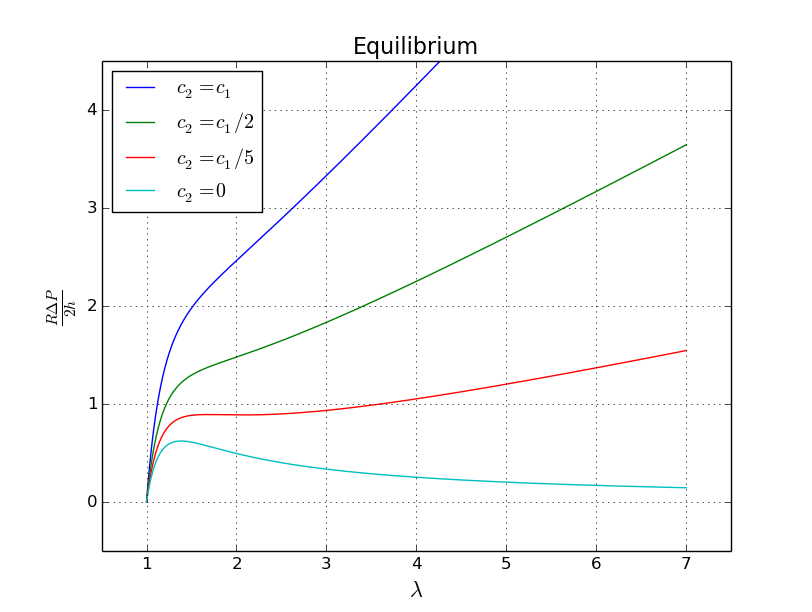
\includegraphics[width=150mm]{figure_2.png}
\caption{The equilibrium condition plotted for $\lambda\in[1,7]$ and for various $c_2$-values.}
\end{figure}
As we can see, the equilibrium condition will have a maximal point if $c_2<c_1/5$, which corresponds situations that are not physical. If we choose $c_2>c_1/5$, all points are physical.
\end{description}
\end{document}
